\documentclass{article}

\usepackage{mathrsfs,amsmath}
\usepackage{xcolor}
\usepackage{titlesec}
\usepackage{listings}
\usepackage{syntax}
\usepackage{pythonhighlighting}

\usepackage{graphicx}

\graphicspath{ {./assets/} }


\usepackage[margin=1.4in]{geometry}

\title{Handout \#7 | CS 471} 
\author{Jared Dyreson\\ 
        California State University, Fullerton}

\DeclareRobustCommand{\bowtie}{%
  \mathrel\triangleright\joinrel\mathrel\triangleleft}


\usepackage [english]{babel}
\usepackage [autostyle, english = american]{csquotes}
\MakeOuterQuote{"}

\titlespacing*{\section}
{0pt}{5.5ex plus 1ex minus .2ex}{4.3ex plus .2ex}
\titlespacing*{\subsection}
{0pt}{5.5ex plus 1ex minus .2ex}{4.3ex plus .2ex}

\usepackage{hyperref}
\hypersetup{
    colorlinks,
    citecolor=black,
    filecolor=black,
    linkcolor=black,
    urlcolor=black
}

\begin{document}

\maketitle
\tableofcontents

\newpage

\section{Questions}

\begin{enumerate}
\item A  packet switch receives a  packet and determines the  outbound link to which the packet should be forwarded. When the packet arrives, one other packet is halfway done being transmitted  on this outbound link  and four other packets are waiting  to be transmitted. Packets are transmitted in order  of arrival. Suppose all packets are 1,500 bytes and the link  rate is 2 MBPS.  What  is the queuing delay  for the  packet? More generally,what  is the  queuing delay when all packets have length L,  the transmission rate  is R, x  bits  of the currently- being-transmitted packet have been transmitted,  and n packets are already in  the queue?
\begin{itemize}
\item Generally the queueing delay can be expressed as the following: \\
$$\text{delay}_{\text{queue}} = \frac{n \times L + (L - x)}{R}$$
\item Therefore, if you plug in the correct values: \\
$$\text{delay}_{\text{queue}} = \frac{4 \times 1500 + (1500 - 750)}{2 \times 10^{6}} = \frac{27}{8000} \text{ seconds } $$
\end{itemize}
\item What does the application layer define?
\begin{itemize}
\item \textbf{Application layer:} specifies the shared communications protocols and interface methods used by hosts in a communications network
\end{itemize}
\begin{figure}[!h]
\centering
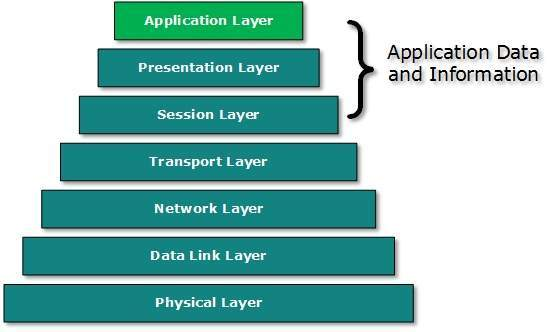
\includegraphics[width=7cm]{application_layer}
\end{figure}
\item What four basic transport layer services may an application need?
\begin{itemize}
\item Data integrity
\item Timing
\item Throughput
\item Security
\end{itemize}
\item I would like to fetch 10 images. How many HTTP requests must my browser send to the server?
\begin{itemize}
\item 11: 1 for the HTML page and 10 for the other resources
\end{itemize}
\newpage
\item For a communication session between a pair of processes, which process is the client and server?

\begin{itemize}
\item Client process: initiates the communication
\item Server process: process that waits to be contacted
\end{itemize}

\item Suppose you wanted to transfer a file from a server to a client as fast as possible. Would you use TCP or UDP?
\begin{itemize}
\item UDP because you are not concerned about the data integrity. You can transmit the data quickly.
\end{itemize}

\item Why do HTTP, FTP, SMTP, and POP3 run over TCP rather than UDP?
\begin{itemize}
\item These protocols use TCP over UDP because of data integrity. All information requested will be collected.
\end{itemize}
\end{enumerate}

\end{document}

